\documentclass[11pt,letterpaper,boxed]{pset}

\usepackage[margin=0.75in]{geometry}
\usepackage{ulem}

\begin{document}

    \problemlist{PHYS051 HW06}
    \begin{center}
        P32.5, E51.44, E33.15, *E33.24, E51.46
    \end{center}
    
    \begin{problem} [P32.5]
    Bainbridge's mass spectrometer, as shown in Fig. 32-39, separates ions having the same velocity. The ions, after entering through slits $S_1$ and $S_2$, pass through a velocity selector composed of an electric field produced by the charged plates P and P', and a magnetic field $\Vec{B}$ perpendicular to the electric field and the ion path. Those ions that pass undeviated through the crossed $\Vec{E}$ and $\Vec{B}$ fields enter into a region where a second magnetic field $\Vec{B'}$ exists, and are bent into circular paths. A photographic plate registers their arrival. Show that $\frac{q}{m}=\frac{E}{rBB'}$, where $r$ is the radius of the circular orbit.
    \end{problem}
    \begin{figure*} [ht]
        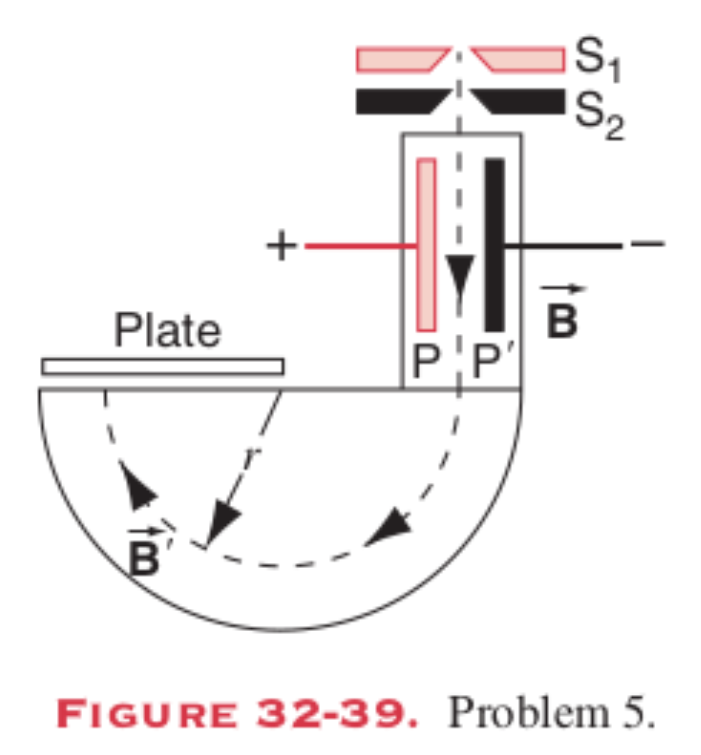
\includegraphics[width=125px]{HW6Images/32-5.png}
        \label{fig:P32-5}
    \end{figure*}
    \newpage
    
    \begin{problem} [E51.44]
    Ordinary water consists of roughly 0.015\% by mass of "heavy water," in which one of the two hydrogens is replaced with deuterium, $^2$H. How much average fusion power could be obtained if we "burned" all the $^2$H in 1 liter of water in 1 day through the reaction $^2$H + $^2$H $\longrightarrow$ $^3$He + n ($Q$ = 3.27 MeV)? (Q refers to the “disintegration energy” of the event, i.e., the energy difference between the initial and final states of the reaction.)
    \end{problem}
    \newpage
    
    \begin{problem} [E33.15]
    Figure 33-43 shows a cross section of a long, thin ribbon of width $w$ that is carrying a uniformly distributed total current $i$ into the page. Calculate the magnitude and the direction of the magnetic field $\Vec{B}$ at the point $P$ in the plane of the ribbon at a distance $d$ from its edge. (Hint: Imagine the ribbon to be constructed from nay long, thin, parallel wires.)
    \end{problem}
    \begin{figure*} [ht]
        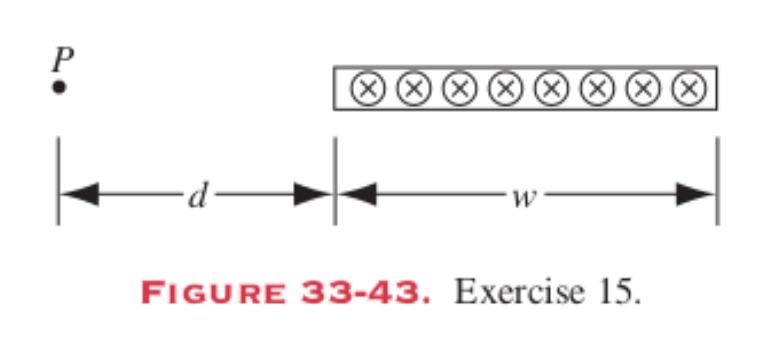
\includegraphics[width=150px]{HW6Images/33-15.png}
        \label{fig:P33-15}
    \end{figure*}
    \newpage
    
    \begin{problem} [*E33.24]
    Figure 33-50 shows a long wire carrying a current $i_1$. The rectangular loop carries a current $i_2$. Calculate the resultant force acting on the loop. Assume that $a$ = 1.10 cm, $b$ = 9.20 cm, $L$ = 32.3 cm, $i_1$ = 28.6 A, and $i_2$ = 21.8 A.
    \end{problem}
    \begin{figure*} [ht]
        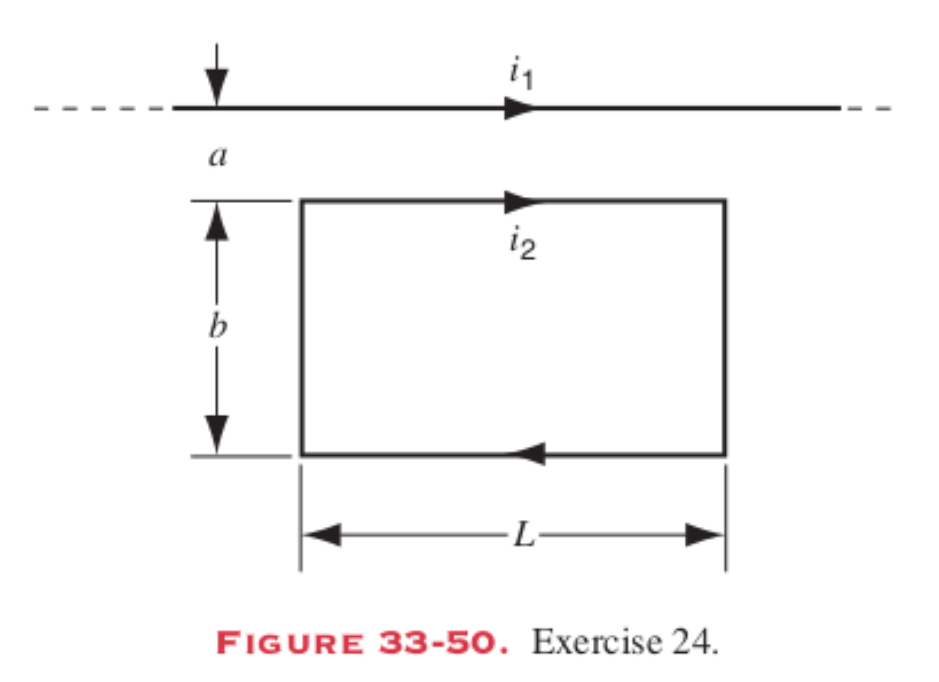
\includegraphics[width=150px]{HW6Images/33-24.png}
        \label{fig:P33-24}
    \end{figure*}
    \newpage
    
    \begin{problem} [E51.46]
    Figure 51.16 shows an idealized representation of a hydrogen bomb. The fusion fuel is lithium deuteride (LiD). The high temperature, particle density, and neutrons to induce fusion are provided by an atomic (fission) bomb "trigger." The fusion reactions are
    
    \begin{multicols} {2}
    $$^6\text{Li} + n \longrightarrow ^3\text{H} + ^4\text{He}$$ \smallskip $$^2\text{H} + ^3\text{H} \longrightarrow ^4\text{He} + n (Q = \text{17.59 MeV})$$
    \end{multicols}
    
    the tritium ($^3$H) produced in the first reaction fusing with the deuterium (D) in the fuel; see Eq. 51-8 [Pg. 1164: $^2\text{H} + ^3\text{H} \longrightarrow ^4\text{He} + n (Q = \text{17.59 MeV})$]. By calculating $Q$ for the first reaction, find the mass of LiD required to produce a fusion yield of 1 megaton of TNT ($=2.6\times10^{28}$ MeV). Needed atomic masses are
    
    \begin{multicols} {2}
    $$^6 \text{Li} = 6.015122 \text{u}$$ $$^4 \text{He} = 4.002603 \text{u}$$
    
    $$^3 \text{H} = 3.016049 \text{u}$$ $$\text{n} = 1.008665 \text{u}$$
    \end{multicols}
    
    \end{problem}
    \begin{figure*} [ht]
        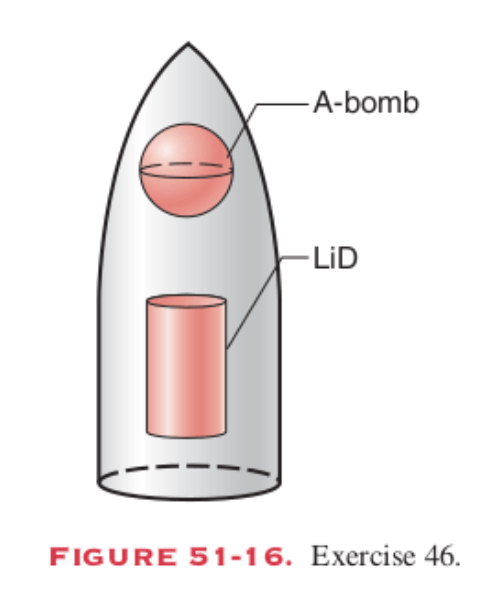
\includegraphics[width=100px]{HW6Images/51-46.png}
        \label{fig:E51-46}
    \end{figure*}
    \newpage
\end{document}